% !TEX encoding = UTF-8 Unicode
% !TEX program = xelatex
% !BIB program = biber
% !TEX TS-program = xelatex
% !BIB TS-program = biber
%%
%%  本模板方式编译: XeLaTeX + biber
%%
%%  注意: 在改变编译方式前应先删除 *.toc 和 *.aux 文件
%%
\documentclass[12pt,openright]{book}

% 引入NKThesis包
\usepackage[emptydoublepage]{NKThesis}   % 中文
%\usepackage[emptydoublepage,English]{NKThesis} % 英文

% 其它包按需添加
% \usepackage{amsmath}
% \usepackage{cases}
% \usepackage{multirow}

% 参考文献
\addbibresource{nkthesis.bib}
% 图片文件夹
\graphicspath{{image/}}

\includeonly{
	./tex/abstract,
	./tex/introduction,
	./tex/relatedwork,
	./tex/method,
	./tex/discussion,
	./tex/summary,
	./tex/references,
	./tex/acknowledgements,
	./tex/appendices,
	./tex/resume
}
\begin{document}

%%%%%%%%%%%%%%%%%%%%%%%%%%%%%%%%%%%%%%%%%%%%%%%%%%%%%%%%%%%%%%%%%%%%%%%%%%%%%%%%
%  设置基本信息
%  注意:  逗号`,'是项目分隔符. 如果某一项的值出现逗号, 应放在花括号内, 如 {,}
%%%%%%%%%%%%%%%%%%%%%%%%%%%%%%%%%%%%%%%%%%%%%%%%%%%%%%%%%%%%%%%%%%%%%%%%%%%%%%%%
\NKTsetup{
	% 封面设置
	论文题目(中文) = 我是爱南开的,
	副标题         = ,
	论文题目(英文) = I Love Nankai,
	论文作者       = 周恩来,
	学号           = 19190062,
	指导教师       = 张伯苓教授,
	申请学位       = 硕士,
	培养单位       = 南开大学,
	学科专业       = 文科,
	研究方向       = 国际政治,
	答辩委员会主席 = {张伯苓},
	评阅人 = {严范孙},
	中图分类号     = ,
	UDC            = ,
	学校代码       = 10055,
	论文完成时间   = 二〇一八年四月,
	% 保密设置
	密级           = 公开,	% 公开 | 限制 | 秘密 | 机密, 若为公开, 不填以下三项
	非公开论文编号 = ,
	保密期限       = ,
	审批表编号     = ,
	% 其他信息
	批准日期       = ,
	答辩日期       = ,
	论文类别       = 学历硕士, % 博士 | 学历硕士 | 专业学位硕士 | 同等学力硕士
	院/系/所       = 文学部,
	联系电话       = 1234567890,
	Email          = ZhouEnlai@nankai.edu.cn,
	通讯地址(邮编) = 300000,
	备注           = {}
}

%%%%%%%%%%%%%%%%%%%%%%%%%%%%
% 论文开始部分
%%%%%%%%%%%%%%%%%%%%%%%%%%%%
% 摘要
% !TeX root = ../main.tex
% -*- coding: utf-8 -*-


\begin{zhaiyao}

深度神经网络(Deep Neural Network, DNN)训练代价昂贵是导致模型知识产权保护问题逐渐被重视的原因。近年来,模型盗窃行为时常出现,不法分子对DNN模型非法复制,派生和发布的行为都严重侵犯了模型所有者的知识产权。许多研究者受到传统数字媒体水印的启发,从而设计模型水印和指纹用于验证模型所有权。然而,歧义性声明等攻击手段被用于破解模型水印和指纹,这对模型所有权验证工作造成了挑战。因此,需要设计一种知识产权保护方法能够解决上述问题。本文通过相关工作的调研,分析目前知识产权保护方法存在的难点与挑战,提出了一种基于近边界数据的模型所有权推断方法,主要工作如下:

1)揭示了当前DNN模型所有权验证方案的脆弱性并确认了数据驱动推断模型所有权的有效性。模型水印和模型指纹的方法通常用是检测嵌入的水印或者通过特定触发集来验证所有权,这种方式在面对歧义攻击击等强攻击时,并不具备很强的鲁棒性。DNN模型通过数据集训练,所以不管是源模型还是其派生出来的模型,总会包含一定数据中的知识,本文确认了数据驱动推断模型所有权方法的有效性。

2)提出了利用对抗性样本构造近边界数据以抵御模型窃取攻击。对抗性样本一般位于模型分类边界上并且相较于其他不相关的模型,对抗性样本可以更好的转移到从原始模型派生出的模型上。因此,本文利用对抗性样本构造了近边界数据来推断模型所有权,抵御模型窃取攻击。

3)设计了基于DCGAN的近边界数据生成器和提出了一种损失函数用以微调源模型的目标分类边界,增加推断模型所有权的置信度。为了防止近边界数据被轻易复制,本文使用DCGAN的生成器生成我们私有的近边界数据。在此基础之上,重新设计了模型损失函数微调源模型,在保持DNN模型性能的情况下,以95\%以上的置信度成功推断模型所有权。

4)本文在三个公开数据集上对本文提出的方法做了详细的测试,实验结果证明了基于近边界数据推断模型所有权的有效性和鲁棒性


\end{zhaiyao}



\begin{guanjianci}
知识产权保护;所有权推断;近边界数据;深度神经网络;生成对抗网络
\end{guanjianci}



\begin{abstract}

Deep Neural Network(DNN) training is expensive, which is why the issue of model intellectual property protection has been increasingly emphasized. In recent years, model theft has been occurring frequently, with malicious actors illegally copying, deriving, and releasing DNN models, which seriously violates the intellectual property of the model owners. Many researchers have been inspired by traditional digital media watermarks and have designed model watermarks and fingerprints to verify model ownership. However, attack methods such as ambiguity declarations have been used to break model watermarks and fingerprints, posing a challenge to model ownership verification. Therefore, a method for protecting intellectual property needs to be designed to address these issues. This paper analyzes the difficulties and challenges of current methods for protecting intellectual property through related work, and proposes a model ownership inference method based on near-boundary data. The main contributions of this work are as follows:

1)We reveal the vulnerability of current DNN model ownership verification schemes and confirm the effectiveness of data-driven inference of model ownership. The methods of model watermark and model fingerprint are usually used to detect embedded watermarks or to verify ownership through specific trigger sets. However, these methods do not have strong robustness in the face of strong attacks such as ambiguity attacks. Since DNN models are trained on a dataset, both the source model and its derivatives will contain some knowledge from the data. This paper confirms the effectiveness of data-driven inference of model ownerships.
 
2)We propose the use of adversarial samples to construct near-boundary data to resist model theft attacks. Adversarial samples are generally located on the model classification boundary and can be better transferred to models derived from the original model compared to other unrelated models. Therefore, this paper uses adversarial samples to construct near-boundary data for ownership inference and to resist model theft attacks.

3)We design a near-boundary data generator based on DCGAN and propose a loss function to fine-tune the target classification boundary of the source model to increase the confidence of ownership inference. In order to prevent near-boundary data from being easily copied, this paper uses a DCGAN generator to generate private near-boundary data. On this basis, the model loss function is redesigned to fine-tune the source model, successfully inferring model ownership with over 95\% confidence while maintaining DNN model performance.

4)We conduct detailed tests on three public datasets to verify the effectiveness and robustness of the proposed method based on near-boundary data for model ownership inference. The experimental results demonstrate  the effectiveness and robustness of ownership inference based on near-boundary data.

\end{abstract}



\begin{keywords}
Intellectual property protection; Ownership inference; Near-boundary data; Deep neural network; Generative adversarial network
\end{keywords} 
% 论文目录
\tableofcontents
% 列出图表目录,如果需要可取消注释
% \listoffigures

%%%%%%%%%%%%%%%%%%%%%%%%%%%%
% 论文主体章节
%%%%%%%%%%%%%%%%%%%%%%%%%%%%
% !TeX root = ../main.tex
% -*- coding: utf-8 -*-

\chapter{绪论}
\label{1}


\section{研究背景与意义}

机器学习的发展

模型知识产权问题描述

模型知识产权相关研究

\section{相关研究现状}

研究问题

研究现状

\section{本文主要工作}

揭示\cite{maini2021dataset}现有问题,确认数据驱动推断所有权的有效性

利用对抗性样本抵御模型窃取

基于DCGAN生成私有数据

广泛实验验证有效性

\section{本文组织架构}

第一章

第二章

第三章

第四章

第五章

第六章
% !TeX root = ../main.tex
% -*- coding: utf-8 -*-


\chapter{技术背景} 
\label{2}

引言

\section{深度神经网络及相关术语}

人工神经网络是一种类似于人类大脑生物神经系统的信息处理模型,它由许多相互连接的神经元(网络中的节点)组成,这些神经元都可以向其他神经元发送信号。一般的神经网络由输入层,隐藏层和输出层组成,如图\ref{深度神经网络结构图}所示,如果一个神经网络有多个隐藏层,那么这个神经网络就被称为深度神经网络。DNN的隐藏层一般由卷积层,池化层,全连接层,Dropout层和Softmax层构成,数据输入输入层后,会经过每一层,每层提取的抽象特征会作为下一层的输入,最终由输出层输出。

\begin{figure}[htbp]%%图,[htbp]是浮动格式
	\centering
	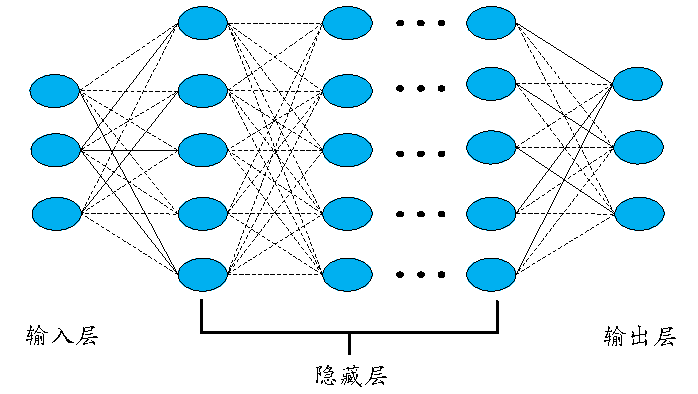
\includegraphics[width=11cm,height=7cm]{深度神经网络结构.pdf}
	%	\centerline{原始样本}
	\setlength{\abovecaptionskip}{5mm} %图片标题与图片距离
	\caption{深度神经网络结构图}
	\label{深度神经网络结构图}
\end {figure}

DNN可以看作是将一组输入变量转化为一组输出变量的非线性数学函数。每个神经元都有对应的权重和偏置参数,控制着输入的精确转化,这些参数在反向传播的过程中,通过损失函数和梯度下降算法来更新。确定这些参数的过程称为DNN模型的学习或者训练,并且需要大量的计算资源,然而权重一旦确定,DNN模型就可以快速的处理相似类型的新数据,识别并提取海量数据中的复杂特征。

以下是本文中涉及到DNN知识产权保护领域中的相关术语:

\begin{enumerate}
	\renewcommand{\labelenumi}{\theenumi)}
	\item 源模型。源模型也称作目标模型,是指模型所有者在私有或公共数据集上,消耗大量计算资源和人力资源训练出的高性能DNN模型,可能因学术研究放置在开源社区,或者作为商用给用户提供远程API。
	\item 可疑模型。可疑模型是指该模型可能是通过模型窃取攻击方法从源模型派生出来的模型,判断一个可疑模型是否是从源模型派生是模型知识产权保护领域的主要目标。
	\item 白盒模式。白盒模式是指能够获得DNN模型的所有知识,包括训练集,训练方式,模型参数,模型结构等。
	\item 黑盒模式。黑盒模式指不清楚模型内部参数,但可以通过模型提供的API获得指定输入的输出。
\end{enumerate}



\section{对抗性攻击}

\subsection{对抗性样本}
 
对抗性样本的概念是Szegedy等人\cite{szegedy2013intriguing}提出的。这篇文章中指出,通常情况下,一个良好性能的DNN模型具备很好的泛化能力,对输入的随机微小扰动具有鲁棒性,因此小扰动不应该改变图像的预测类别。然而,对图像添加特定的非随机扰动,使得损失函数的值增大,可以任意改变DNN模型的预测结果。这种人类肉眼上难以察觉但可以使模型输出错误类别的样本称为对抗性样本。 

用$f:R^m \rightarrow {1,2,...,n}$表示将一张图片映射为$n$个标签的DNN分类器,对一个正常样本$x \in R^m$以及一个错误标签$l$,目标是找到一个最小的扰动$\delta$,使得分类器将样本$x$错误分类为$l$,如式\ref{eq:1}所示:
\begin{equation}
	\label{eq:1}
	\begin{split}
	&min\parallel \delta \parallel_2, \\
	 &s.t. \ f(x + \delta) = l,\ x + \delta \in [0,1]^m
	\end{split}
\end{equation}
其中叠加了扰动的$x +\delta$即为一个对抗性样本。\ref{eq:1}这种方式通常用在黑盒的场景下,仅根据DNN分类器的输出进行扰动$\delta$的调整。
 
 在白盒场景下,由于知道模型的所有知识,可以根据这些信息来寻找对抗性样本,通常利用DNN分类器的损失函数来寻找对抗性样本。
 
 用$f:R^m \rightarrow {1,2,...,n}$表示将一张图片映射为$n$个标签的DNN分类器,对一个正常样本$x \in R^m$以及它对应的正确标签$y$,目标是找到一个足够小小的扰动$\delta:\delta \leq \gamma$,使得加上扰动后的样本输入DNN模型后,损失函数$L$达到最大值,如式\ref{eq:2}所示:
 \begin{equation}
 	\label{eq:2}
 		\delta = arg \mathop{max} \limits_{\delta \leq \gamma} L(f(\theta, x + \delta), y)
\end{equation}
其中$\theta$是分类器$f$的参数,$x + \delta$是一个扰动后的对抗性样本。
 
 \subsection{对抗性攻击的类别}

对抗性攻击技术是指生成对抗性样本的方法,不同的方法生成对抗性样本的效率,质量也不相同。根据方式的不同,可以分为以下几类:

\begin{enumerate}
	\renewcommand{\labelenumi}{\theenumi)}
	\item 白盒攻击与黑盒攻击。白盒攻击指敌手知道DNN模型的参数和内部结构等信息,利用这些信息发起的攻击。黑盒攻击指敌手仅根据模型的输入输出来发起攻击。
	\item 有目标攻击和无目标攻击。有目标攻击指对抗性样本的预测类别为敌手指定的类别,例如将一张牛的图片识别为羊,而不能是其他类别,常采取的方式是向各个方向搜索扰动来最大化DNN模型预测特定类上的可能性。无目标攻击指添加扰动来改变原始预测类别,对具体分类类别不做要求。通常来说有两种攻击方式,一种是最小化DNN模型预测正确类的可能性,一种是进行多次不同类别的的有目标攻击,然后在多个对抗性样本中选取扰动最小的。
	\item 单步攻击和迭代攻击。单步攻击指通过一次添加扰动生成对抗性样本,迭代攻击指通过多次迭代添加微小扰动来生成对抗性样本。通常来说迭代攻击的成功率较高,但是相应的算法复杂度更高,效率较低。
	\item 个体攻击和普适性攻击。个体攻击指针对每个样本都需要重新生成扰动,普适性攻击指找到一个通用的扰动,对数据集中的一类数据都叠加该扰动,普适性攻击效率较高,但是寻找通用扰动的难度较大。
\end{enumerate}

\section{生成对抗网络}

Goodfellow等人\cite{goodfellow2014generative}第一次提出了生成对抗网络(Generative Adversarial Network, GAN),GAN由一个生成器和一个判别器构成,

\begin{figure}[htbp]%%图,[htbp]是浮动格式
	\centering
	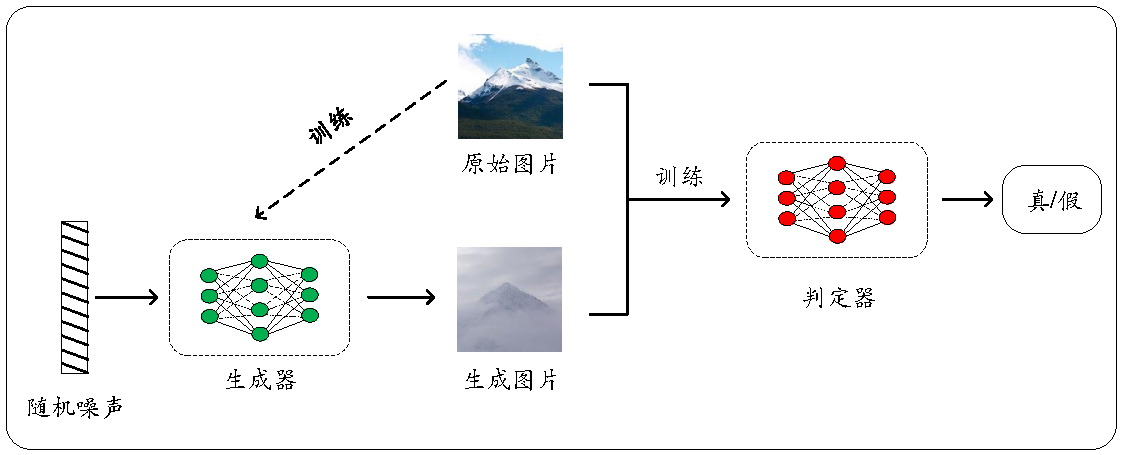
\includegraphics[width=14.5cm,height=7cm]{生成对抗网络结构.pdf}
	%	\centerline{原始样本}
	\setlength{\abovecaptionskip}{5mm} %图片标题与图片距离
	\caption{生成对抗网络结构图}
	\label{生成对抗网络结构图}
\end {figure}






\section{深度神经网络模型窃取攻击}

深度神经网络模型窃取攻击相关概念


\section{深度神经网络模型的知识产权保护}


深度神经网络模型的知识产权保护相关概念


\section{本章小结}


小结

% !TeX root = ../main.tex
% -*- coding: utf-8 -*-

\chapter{常用包}
\label{chpt:method}

\section{The Tikz 绘图Package}
\label{sec:method:tikz}


The {\scshape pdf}\ package, where ``{\scshape pdf}'' is supposed to mean ``portable
graphics format'' (or ``pretty, good, functional'' if you
prefer\dots), is a package for creating graphics in an ``inline''
manner. It defines a number of \TeX\ commands that draw
graphics. For example, the code \verb|\tikz \draw (0pt,0pt) -- (20pt,6pt);|
yields the line \tikz \draw (0pt,0pt) -- (20pt,6pt); and the code \verb|\tikz \fill[orange] (1ex,1ex) circle (1ex);| yields \tikz
\fill[orange] (1ex,1ex) circle (1ex);.

\begin{figure}[h]
    \centering
    % !TeX root = ../main.tex

\begin{tikzpicture}[->,>=stealth,shorten >=1pt,auto,node distance=2.8cm,semithick]
  \tikzstyle{every state}=[fill=yellow,draw=none,text=black]

  \node[state]         (S) at (-6, 0)              {$S$};
  \node[state]         (xin1) at (-2, 3)           {$X^1_{in}$};
  \node[state]         (xin2) at (-2, 1)        {$X^2_{in}$};
  \node[state]         (xin3) at (-2, -1)       {$X^3_{in}$};
  \node[state]         (xin4) at (-2, -3)           {$X^4_{in}$};
  \node[state]         (xout1) at (0, 3)          {$X^1_{out}$};
  \node[state]         (xout2) at (0, 1)        {$X^2_{out}$};
  \node[state]         (xout3) at (0, -1)   {$X^3_{out}$};
  \node[state]         (xout4) at (0, -3)           {$X^4_{out}$};
  \node[state]         (xin5)  at (3, -2)   {$X^5_{in}$};
  \node[state]         (xout5) at (5, -2)   {$X^5_{out}$};
  \node[state]         (DC) at (7, 2)           {$DC$};

  \path (S) edge[bend left=26]              node {$\infty$} (xin1)
            edge[bend left=12]              node {$\infty$} (xin2)
            edge[bend right=12]             node {$\infty$} (xin3)
            edge[bend right=26]             node {$\infty$} (xin4)
        (xin1) edge  node {$\alpha=1$} (xout1)
        (xin2) edge  node {$\alpha=1$} (xout2)
        (xin3) edge  node {$\alpha=1$} (xout3)
        (xin4) edge  node {$\alpha=1$} (xout4)
        (xin5) edge  node {$1$} (xout5);
  \draw[->] (xout1) to[out=-30,in=150] node {$\beta$} (xin5);
  \draw[->] (xout2.east) to[out=-15,in=165] node [below] {$\beta$} (xin5);
  \draw[->] (xout3.east) to[out=0,in=180] node [below] {$\beta$} (xin5.west);
  \draw[->] (xout1) to[out=-5,in=175] node {$\infty$} (DC);
  \draw[->] (xout5) to[out=40, in=-120] node {$\infty$} (DC);
\end{tikzpicture}
 
    \caption{\label{fig:exmaple1} 示例图1}
\end{figure}

In a sense, when you use {\scshape pdf}\ you ``program'' your graphics, just
as you ``program'' your document when you use \TeX.  You get all
the advantages of the ``\TeX-approach to typesetting'' for your
graphics: quick creation of simple graphics, precise positioning, the
use of macros, often superior typography. You also inherit all the
disadvantages: steep learning curve, no \textsc{wysiwyg}, small
changes require a long recompilation time, and the code does not
really ``show'' how things will look like.





\begin{figure}
    \centering
    % !TeX root = ../main.tex

\begin{tikzpicture}[node distance=2cm]
 %定义流程图具体形状
 \tikzstyle{startstop} = [rectangle, rounded corners, minimum width=3cm, minimum height=1cm,text centered, draw=black, fill=red!30]
 \tikzstyle{io} = [trapezium, trapezium left angle=70, trapezium right angle=110, minimum width=3cm, minimum height=1cm, text centered, draw=black, fill=blue!30]
 \tikzstyle{process} = [rectangle, minimum width=3cm, minimum height=1cm, text centered, draw=black, fill=orange!30]
 \tikzstyle{decision} = [diamond, minimum width=3cm, minimum height=1cm, text centered, draw=black, fill=green!30]
 \tikzstyle{arrow} = [thick,->,>=stealth]
 
\node (start) [startstop] {Start};
\node (in1) [io, below of=start] {Input};
\node (pro1) [process, below of=in1] {Process 1};
\node (dec1) [decision, below of=pro1, yshift=-0.5cm] {Decision 1};
\node (pro2a) [process, below of=dec1, yshift=-0.5cm] {Process 2a};
\node (pro2b) [process, right of=dec1, xshift=2cm] {Process 2b};
\node (out1) [io, below of=pro2a] {Output};
\node (stop) [startstop, below of=out1] {Stop};
 
 %连接具体形状
\draw [arrow](start) -- (in1);
\draw [arrow](in1) -- (pro1);
\draw [arrow](pro1) -- (dec1);
\draw [arrow](dec1) -- (pro2a);
\draw [arrow](dec1) -- (pro2b);
\draw [arrow](dec1) -- node[anchor=east] {yes} (pro2a);
\draw [arrow](dec1) -- node[anchor=south] {no} (pro2b);
\draw [arrow](pro2b) |- (pro1);
\draw [arrow](pro2a) -- (out1);
\draw [arrow](out1) -- (stop);
\end{tikzpicture}

    \caption{\label{fig:exmaple2} 示例流程图2}
\end{figure}


\section{代码块}
\label{sec:method:code}

python 代码可以直接使用\textbf{python}环境

\begin{python}[caption={斐波那契Python}]
def fibonacci(n):
    # Fibonacci number
    if n < 0:
        return False
    if n <= 1:
        return n
    return fibonacci(n-2) + fibonacci(n-1)
\end{python}

C/C++ 代码可以直接使用\textbf{cpp}环境

\begin{cpp}[caption={斐波那契C++}]
unsigned long Fibonacci(int n)
{
    // Fibonacci start from 0
    if (n <= 1) 
    {
        return n;
    }
    else 
    {
        return Fibonacci(n - 1) + Fibonacci(n - 2);
    }
}
\end{cpp}

其他代码,使用\textbf{lstlisting}指明 \textbf{language}即可,如matlab代码

\begin{lstlisting}[caption={Matlab代码},language=Matlab]
function a = factorial(n)
% return n!
    if n==0
        a=1;
    else
        a=n * factorial(n-1);
    end
\end{lstlisting}
% !TeX root = ../main.tex
% -*- coding: utf-8 -*-

\chapter{基于近边界数据的模型所有权推断方法分析}\label{5}

我们在开源数据集CIFAR-10\cite{krizhevsky2009learning},Heritage\cite{Heritage},Intel\_image\cite{Intel_image}上面进行实验,并选择ResNet18作为评估的源模型,VGG11作为对照的无关模型。本文使用的模型均在开源的预训练模型上进行训练。

\noindent\textbf{被盗模型:}我们设置了常见的几种模型盗窃方法,包括模型微调,模型剪枝(不同的剪枝率)和模型蒸馏,并在源模型的基础上得到被盗模型。

\section{实验设置}\label{5.1}

本文实验利用CIFAR-10,Heritage和Intel\_image三种数据集训练ResNet18,训练过程中Adam优化器并将学习率(Learning rate),迭代轮次(Epoch)和每批次大小(Batch size)分别设置为0.0001,200和64。蒸馏模型实验选择从Resnet18蒸馏至VGG11,蒸馏时将蒸馏温度设置为20并且教师模型比例$\alpha$=0.7,训练轮次是20。初始近边界数据生成采用$CW$-$L_2$算法,实验中选择有目标的生成方式,且学习率,迭代次数和二分搜索次数分别设置为0.001,1000和6,其他参数为默认值。私有近边界数据生成器采用DCGAN的基础结构,训练过程使用Adam优化器且将学习率,训练轮次和每批次大小分别设置为0.0002,8000和64。注意本发明最后微调源模型阶段需要交替使用源模型损失函数和微调目标边界的损失函数来微调源模型,具体设置为10个轮次交替一次且交替次数最多为10次。



\section{生成初始近边界数据的算法选择}\label{5.2}

本小节将对\ref{3}\ref{3.2}中提出的FGSM,IGSM,RFGSM和CW-$L_2$进行测试,我们均使用原作者发布的实现。FGSM,IGSM,RFGSM中均有一个用于界定噪声$\epsilon$的参数,且IGSM和RFGSM还包含一个重要的参数$\alpha$ 用来表示迭代次数。我们进行大量的实验探索选择合适的参数用于与CW-$L_2$进行比较。此外,CW-$L_2$的实验设置如\ref{5.1}所示。如表\ref{table:1}所示,CW-$L_2$生成的对抗性样例与目标分类边界的平均距离远比其他算法小。因此,本文使用该算法作为初始近边界数据生成算法。

\begin{table}[H]
	\centering
	\setlength{\arrayrulewidth}{0.5mm}
	\renewcommand\arraystretch{1.5}
	\caption{不同对抗性样本生成算法生成的数据与目标分类边界的平均距离}
	\label{table:1}
	\begin{tabular*}{13cm}{@{\extracolsep{\fill}} l c c c c}
		
		\hline
		数据集                    &   FGSM   &   IGSM   &  RFGSM  &   CW-$L_2$    \\
		\hline
\multirow{3}{6em}{CIFAR-10}      &    0.557  &   0.430  &  0.418   &    0.066     \\
		                         &    0.461  &   0.419  &  0.373   &    0.103     \\
		                         &    0.586  &   0.369  &  0.356   &    0.112     \\
		\hline
\multirow{3}{6em}{Heritage}      &    0.347  &   0.356  &  0.314   &    0.014     \\
		                         &    0.277  &   0.340  &  0.281   &    0.016     \\
		                         &    0.348  &   0.332  &  0.276   &    0.010     \\
		\hline
\multirow{3}{6em}{Intel\_image}  &    0.522  &   0.447  &  0.353   &    0.088     \\
		                         &    0.475  &   0.506  &  0.387   &    0.122     \\
		                         &    0.468  &   0.402  &  0.428   &    0.127     \\
		\hline		
	\end{tabular*}
\end{table}


\section{数据近边界特性的评估与扩展}\label{5.3}

\begin{figure}[htbp]%%图,[htbp]是浮动格式
	\centering
	\begin{minipage}[htbp]{0.49\linewidth}        %图片占用一行宽度的50%
		\hspace{2mm}
		\centering
		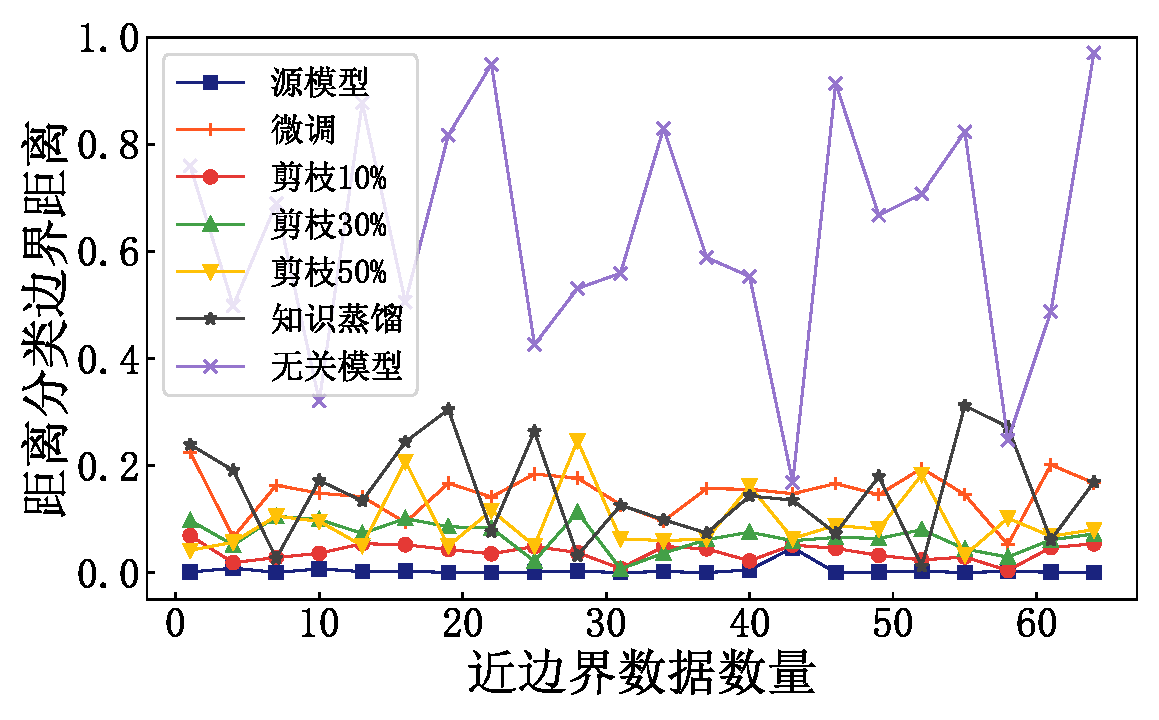
\includegraphics[width=7cm,height=4cm]{CIFAR-10-4-2-distance}
		\centerline{分类边界1}
	\end{minipage}
	\begin{minipage}[htbp]{0.49\linewidth}        %图片占用一行宽度的50%
		\hspace{2mm}
		\centering
		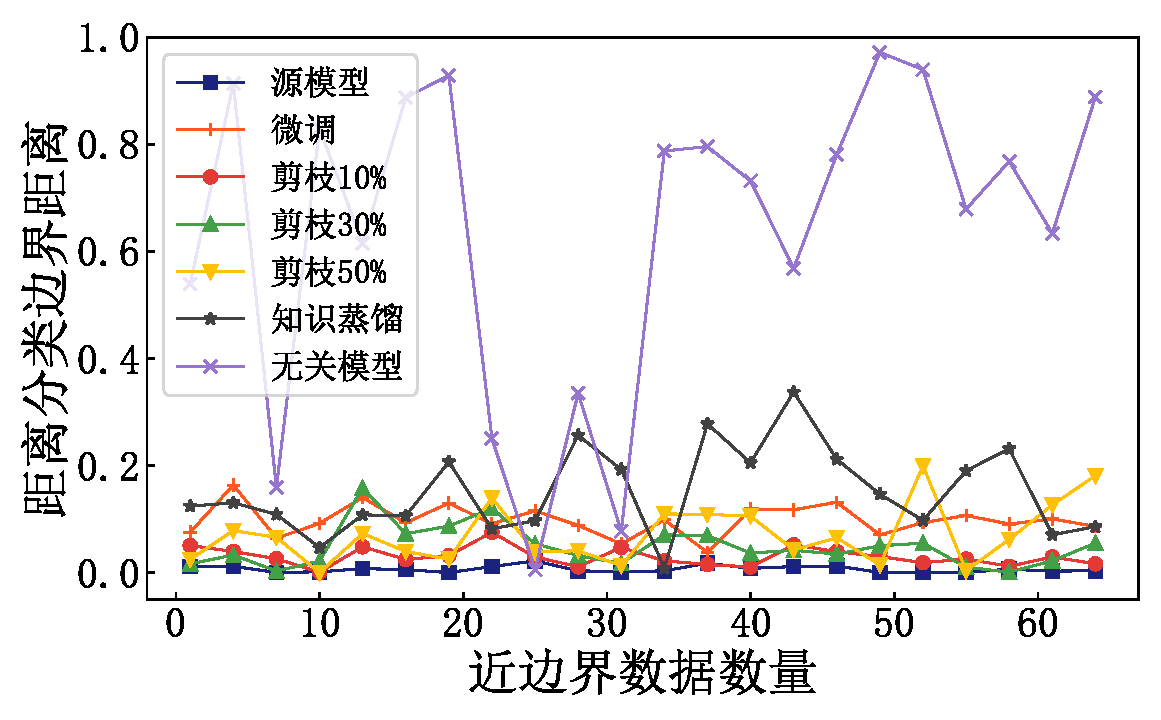
\includegraphics[width=7cm,height=4cm]{CIFAR-10-4-3-distance}
		\centerline{分类边界2}
	\end{minipage}
	\begin{minipage}[htbp]{0.49\linewidth}        %图片占用一行宽度的50%
		\hspace{2mm}
		\centering
		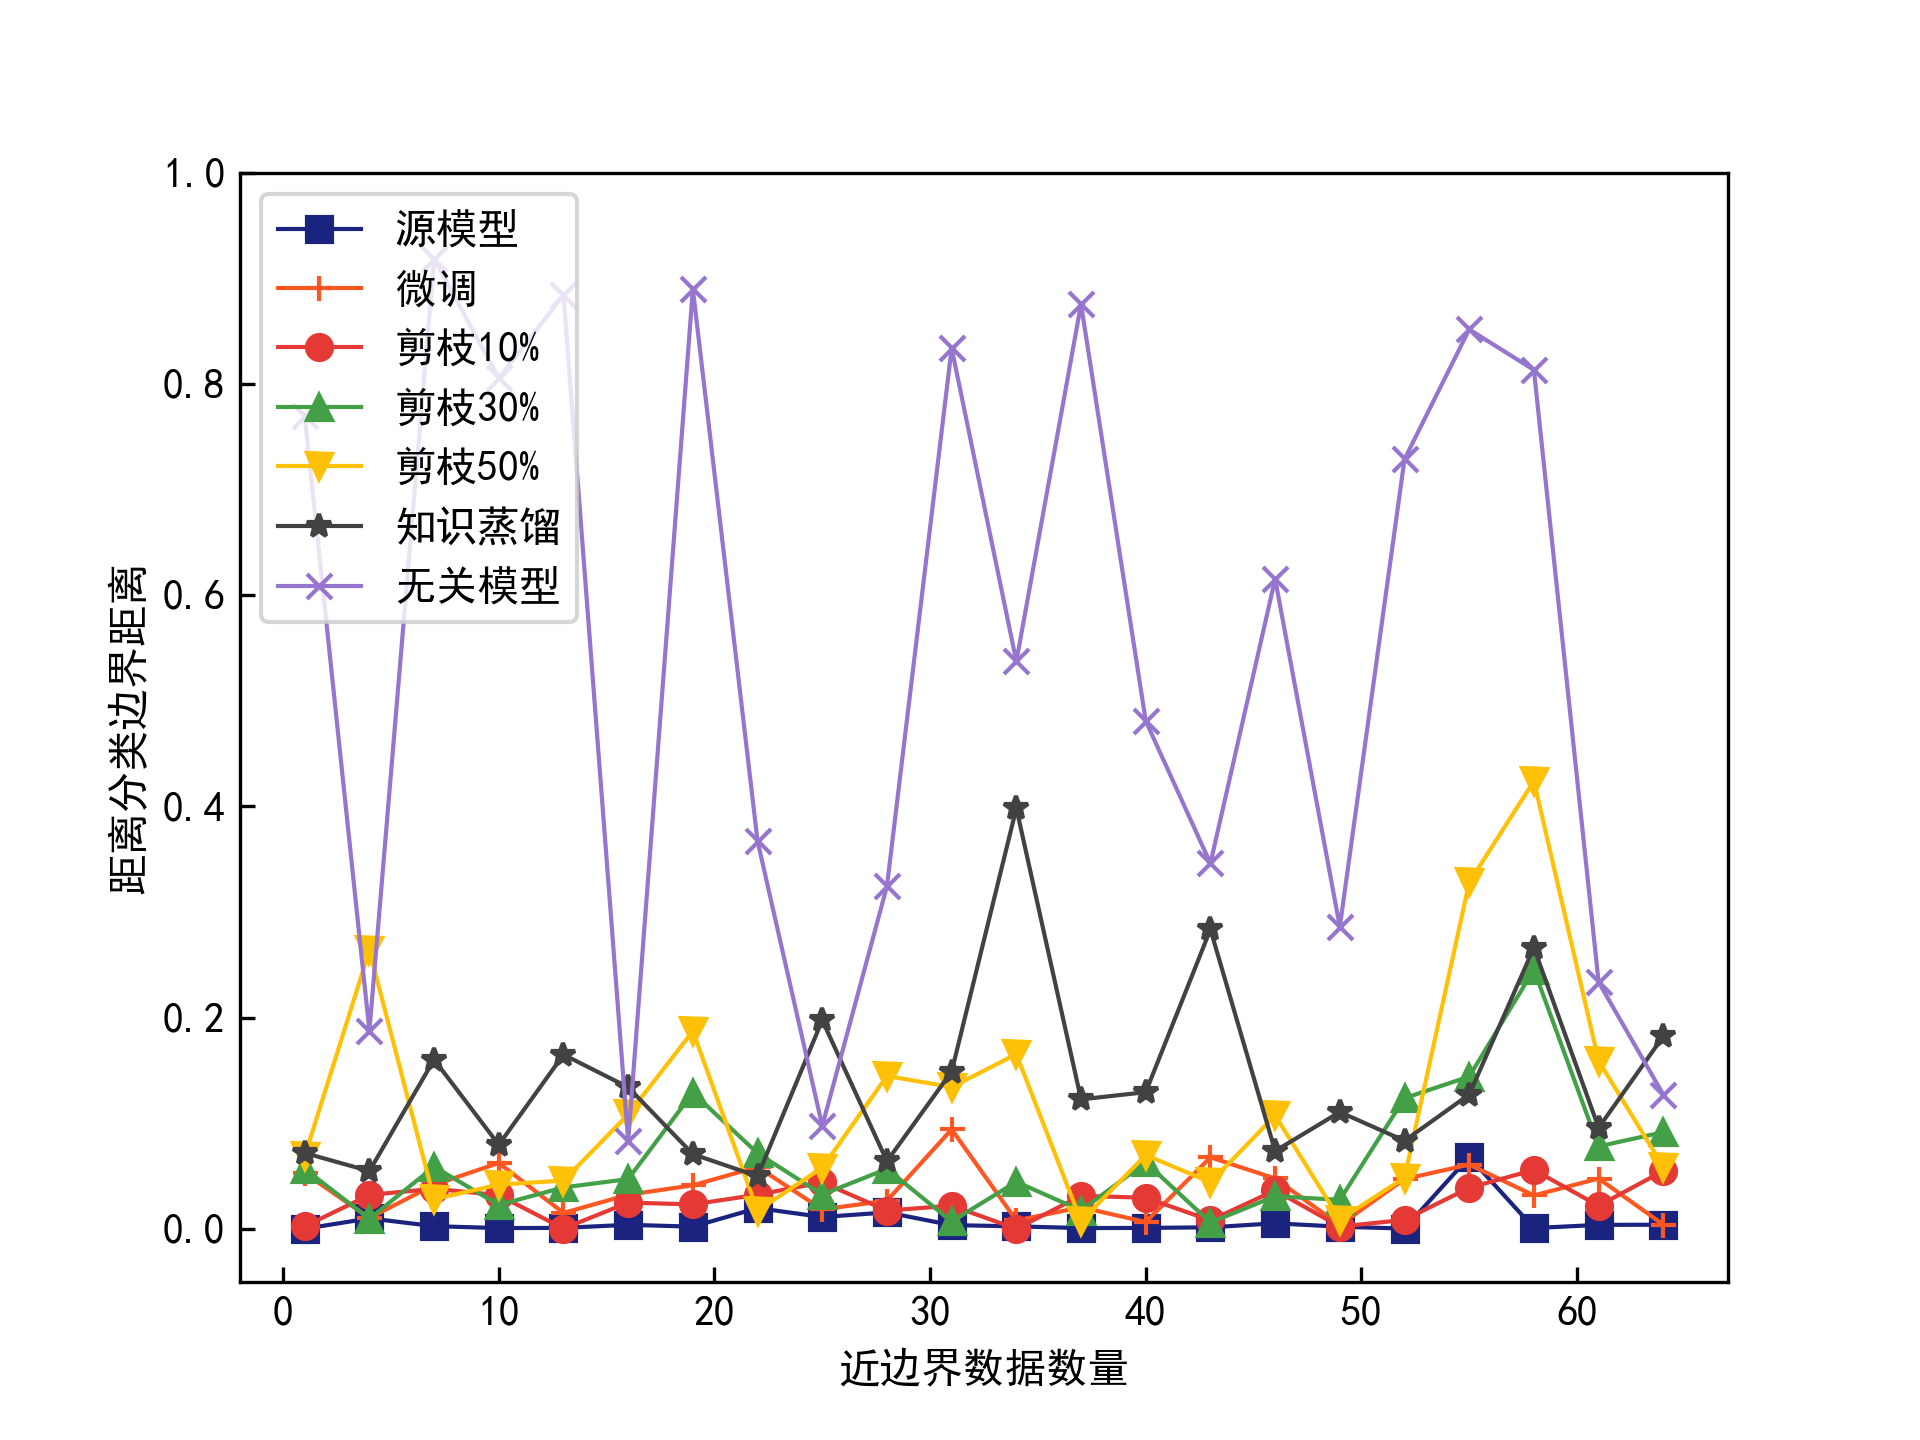
\includegraphics[width=7cm,height=4cm]{CIFAR-10-4-7-distance}
		\centerline{分类边界3}
	\end{minipage}
	\begin{minipage}[htbp]{0.49\linewidth}        %图片占用一行宽度的50%
		\hspace{2mm}
		\centering
		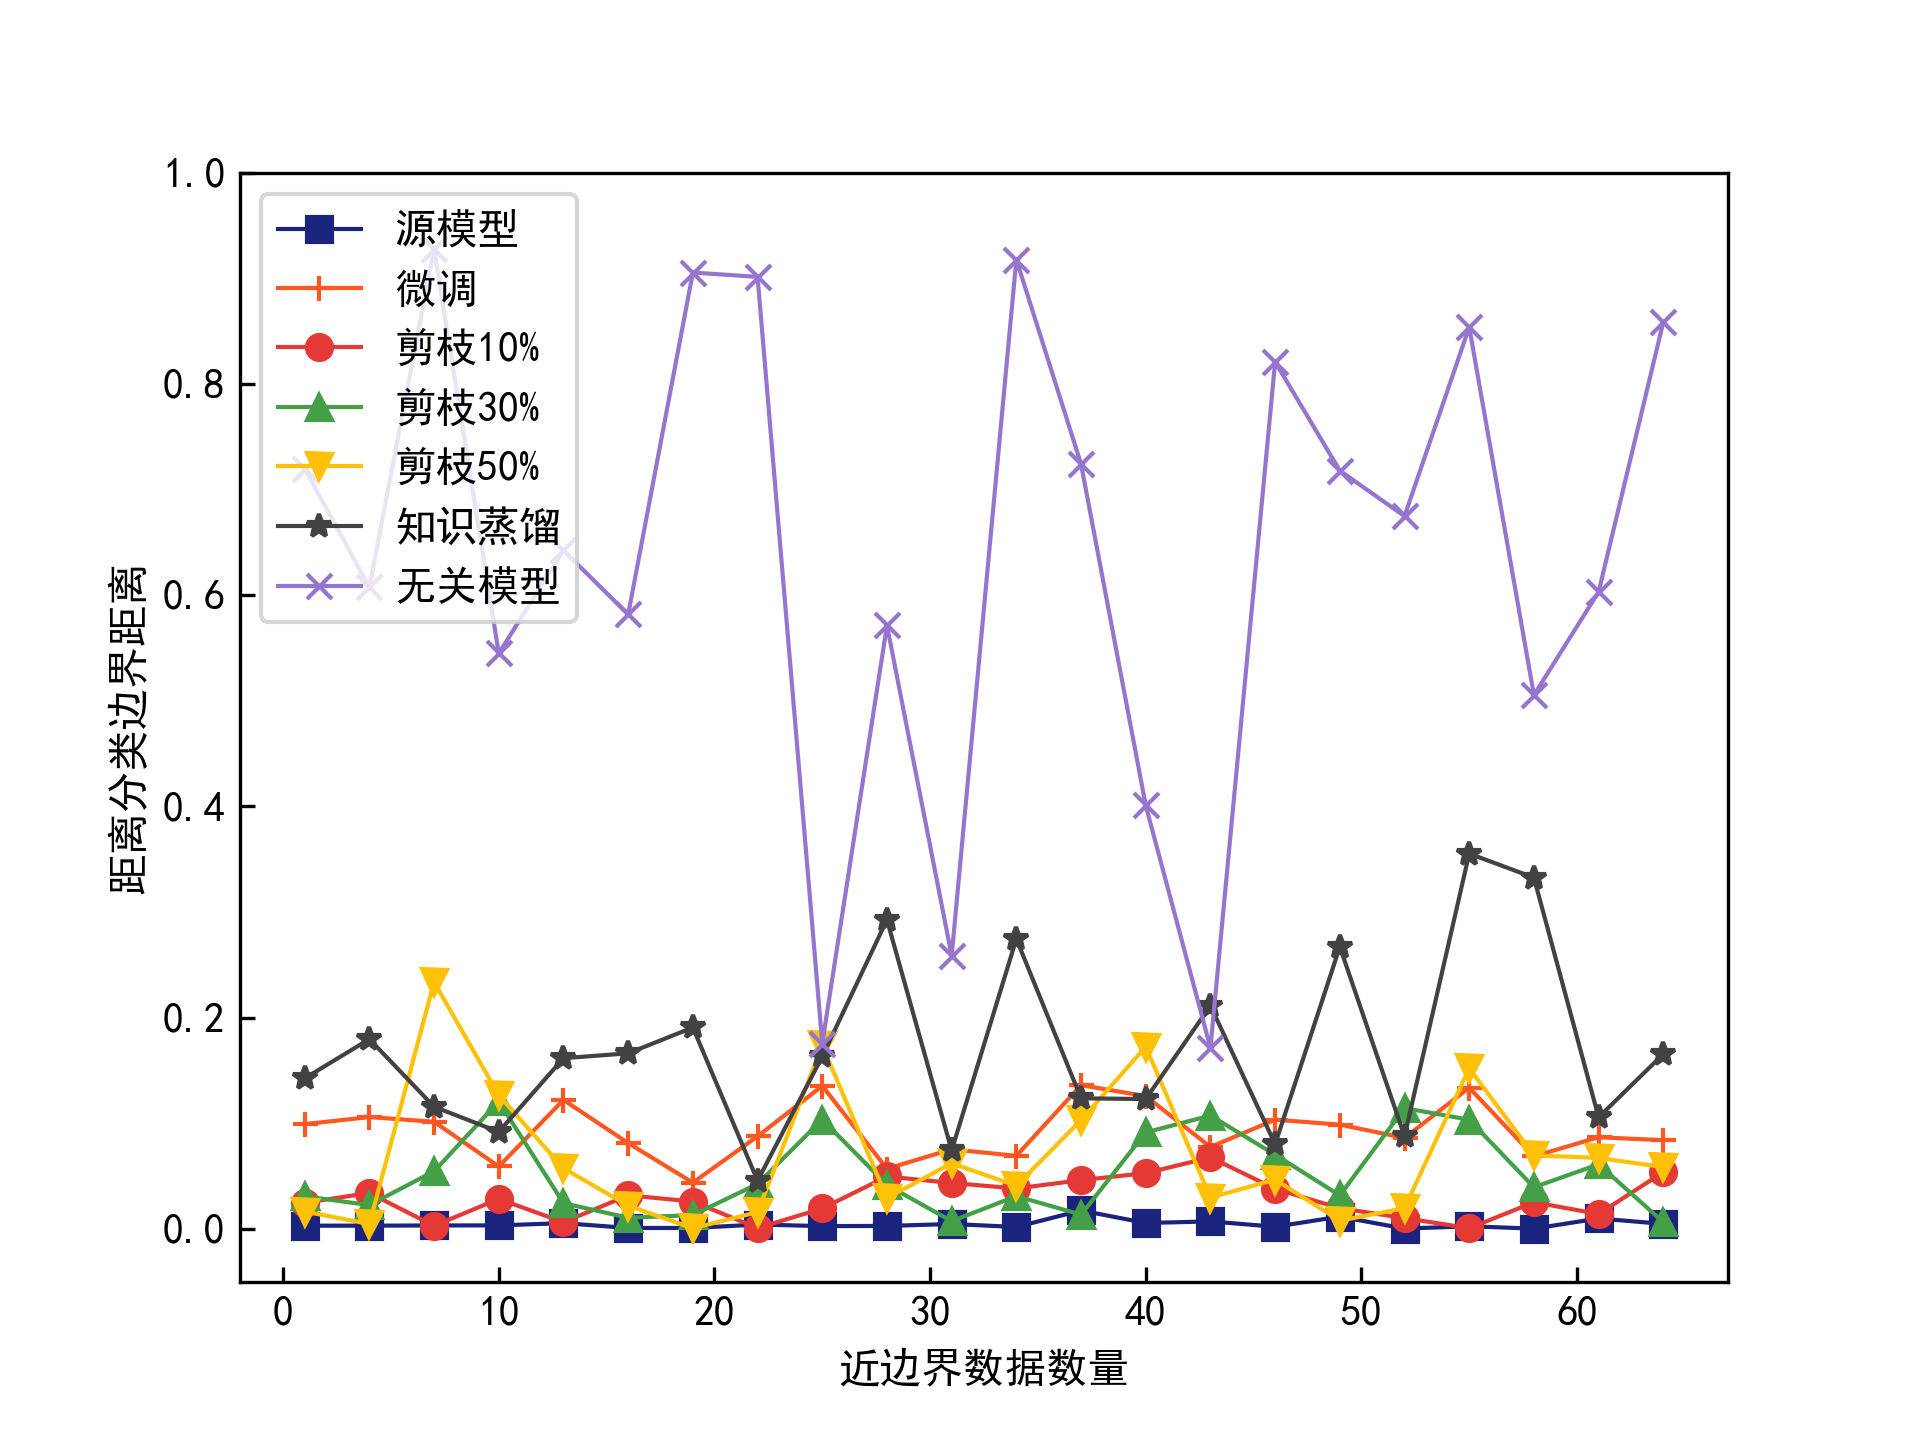
\includegraphics[width=7cm,height=4cm]{CIFAR-10-5-6-distance}
		\centerline{分类边界4}
	\end{minipage}
\setlength{\abovecaptionskip}{7mm} %图片标题与图片距离
\caption{原始样本与对抗性样本对比}
\label{原始样本与对抗性样本对比1}
\end {figure}


\section{推断模型所有权}\label{5.4}

\begin{table}[H]
	\centering
	\setlength{\arrayrulewidth}{0.5mm}
	\renewcommand\arraystretch{1.5}
	\caption{推断模型所有权}
	\label{table:2}
	\resizebox{\linewidth}{!}{
	\begin{tabular}{l l c c c c c c c c c c}
		
		\hline
\multirow{2}{5em}{数据集}&\multirow{2}{4em}{攻击方法}&\multicolumn{2}{c}{分类边界1}&\multicolumn{2}{c}{分类边界2}&\multicolumn{2}{c}{分类边界3}&\multicolumn{2}{c}{分类边界4}&\multicolumn{2}{c}{分类边界5}\\ \cline{3-12}
		                         & &$\Delta\mu$&$p$值&$\Delta\mu$&$p$值&$\Delta\mu$&$p$值&$\Delta\mu$&$p$值&$\Delta\mu$&$p$值 \\
		\hline
\multirow{6}{5em}{CIFAR-10}     &源模型    & 0.913 & $10^{-6}$ & 0.954 & $10^{-6}$ & 0.927 & $10^{-5}$ & 0.967 & $10^{-5}$ & 0.958 & $10^{-5}$   \\
								&模型微调  & 0.718 & $10^{-5}$ & 0.745 & $10^{-6}$ & 0.698 & $10^{-5}$ & 0.692 & $10^{-4}$ & 0.729 & $10^{-5}$   \\
								& 剪枝10\% & 0.572 & $10^{-5}$ & 0.487 & $10^{-5}$ & 0.458 & $10^{-5}$ & 0.533 & $10^{-4}$ & 0.512 & $10^{-4}$   \\
								&剪枝30\%  & 0.537 & $10^{-4}$ & 0.497 & $10^{-4}$ & 0.401 & $10^{-3}$ & 0.428 & $10^{-4}$ & 0.587 & $10^{-4}$   \\
								&剪枝50\%  & 0.545 & $10^{-4}$ & 0.614 & $10^{-4}$ & 0.506 & $10^{-3}$ & 0.570 & $10^{-4}$ & 0.484 & $10^{-3}$   \\
								&知识蒸馏  & 0.372 & $10^{-3}$ & 0.297 & $10^{-3}$ & 0.288 & $10^{-3}$ & 0.308 & $10^{-3}$ & 0.340 & $10^{-3}$   \\
		\hline
\multirow{6}{5em}{Heritage}     &源模型    & 0.876 & $10^{-5}$ & 0.845 & $10^{-5}$ & 0.859 & $10^{-4}$ & 0.801 & $10^{-4}$ & 0.837 & $10^{-5}$   \\
								&模型微调  & 0.815 & $10^{-5}$ & 0.792 & $10^{-4}$ & 0.824 & $10^{-4}$ & 0.833 & $10^{-4}$ & 0.784 & $10^{-4}$   \\
								&剪枝10\%  & 0.530 & $10^{-4}$ & 0.535 & $10^{-3}$ & 0.508 & $10^{-4}$ & 0.486 & $10^{-3}$ & 0.471 & $10^{-3}$   \\
								&剪枝30\%  & 0.491 & $10^{-3}$ & 0.452 & $10^{-3}$ & 0.469 & $10^{-4}$ & 0.470 & $10^{-3}$ & 0.427 & $10^{-4}$   \\
								&剪枝50\%  & 0.502 & $10^{-3}$ & 0.517 & $10^{-3}$ & 0.434 & $10^{-3}$ & 0.451 & $10^{-3}$ & 0.490 & $10^{-3}$   \\
								&知识蒸馏  & 0.329 & $10^{-3}$ & 0.365 & $10^{-2}$ & 0.238 & $10^{-3}$ & 0.310 & $10^{-3}$ & 0.274 & $10^{-3}$   \\
		\hline
\multirow{6}{5em}{Intel\_image} &源模型    & 0.859 & $10^{-5}$ & 0.896 & $10^{-4}$ & 0.872 & $10^{-4}$ & 0.899 & $10^{-4}$ & 0.914 & $10^{-4}$   \\
								&模型微调  & 0.717 & $10^{-5}$ & 0.784 & $10^{-4}$ & 0.752 & $10^{-4}$ & 0.791 & $10^{-3}$ & 0.709 & $10^{-4}$   \\
								&剪枝10\%  & 0.451 & $10^{-4}$ & 0.522 & $10^{-4}$ & 0.539 & $10^{-3}$ & 0.472 & $10^{-3}$ & 0.438 & $10^{-4}$   \\
								&剪枝30\%  & 0.407 & $10^{-4}$ & 0.415 & $10^{-4}$ & 0.346 & $10^{-3}$ & 0.382 & $10^{-3}$ & 0.395 & $10^{-3}$   \\
								&剪枝50\%  & 0.370 & $10^{-3}$ & 0.395 & $10^{-3}$ & 0.327 & $10^{-3}$ & 0.360 & $10^{-3}$ & 0.458 & $10^{-3}$   \\
								&知识蒸馏  & 0.336 & $10^{-2}$ & 0.395 & $10^{-3}$ & 0.360 & $10^{-2}$ & 0.308 & $10^{-3}$ & 0.287 & $10^{-2}$   \\
		\hline		
	\end{tabular}
}
\end{table}



\section{微调目标分类边界的影响}\label{5.5}

\begin{table}[H]
	\centering
	\setlength{\arrayrulewidth}{0.5mm}
	\renewcommand\arraystretch{1.8}
	\caption{微调分类边界对模型的影响}
	\label{table:state}
	\begin{tabular*}{13cm}{@{\extracolsep{\fill}} l c c}
		
	\hline
	数据集        &    微调前准确率   &   微调后准确率            \\
	\hline
	CIFAR-10      &     0.886        &     0.873               \\
	
	Heritage      &     0.879        &     0.856               \\
	
	Intel\_image  &     0.794        &     0.786               \\
	\hline		
	\end{tabular*}
\end{table}

\begin{table}[H]
	\centering
	\setlength{\arrayrulewidth}{0.5mm}
	\renewcommand\arraystretch{1.2}
	\caption{CIFAR-10上不同对抗性样本生成算法生成的数据与目标分类边界的平均距离}
	\label{table:3}
	\begin{tabular*}{14cm}{@{\extracolsep{\fill}} l l c c}
		
		\hline
		数据集 \ (准确率)   &   分类边界   &  数据数量  &   微调后准确率    \\
		\hline
\multirow{20}{8em}{CIFAR-10\ (0.886)}         &\multirow{4}{6em}{分类边界1}&  64   & 0.873    \\
								              &                           &  128  & 0.862     \\
								              &                           &  256  & 0.862     \\
								              &                           &  512  & 0.854     \\
		\cline{2-4}						   
								              &\multirow{4}{6em}{分类边界2} &  64  & 0.871 \\
								              &                            &  128 & 0.870     \\
								              &                            &  256 & 0.860     \\
								              &                            &  512 & 0.844     \\
		
		\cline{2-4}						       
											  &\multirow{4}{6em}{分类边界3} & 64   & 0.871  \\
											  &                            &  128 & 0.868     \\
											  &                            &  256 & 0.858     \\
											  &                            &  512 & 0.856     \\
		\cline{2-4}						       
											  &\multirow{4}{6em}{分类边界4} & 64   & 0.873  \\
											  &                            &  128 & 0.873     \\
											  &                            &  256 & 0.866     \\
											  &                            &  512 & 0.862     \\
		\cline{2-4}						       
											  &\multirow{4}{6em}{分类边界5} & 64  & 0.876  \\
											  &                            & 128 & 0.866     \\
											  &                            & 256 & 0.868     \\
											  &                            & 512 & 0.861     \\
		\hline	
	\end{tabular*}
\end{table}

\begin{table}[H]
	\centering
	\setlength{\arrayrulewidth}{0.5mm}
	\renewcommand\arraystretch{1.2}
	\caption{Heritage上不同对抗性样本生成算法生成的数据与目标分类边界的平均距离}
	\label{table:4}
	\begin{tabular*}{14cm}{@{\extracolsep{\fill}} l l c c}
		
		\hline
		数据集 \ (准确率)   &   分类边界   &  数据数量  &   微调后准确率    \\
		\hline
		\multirow{20}{8em}{Heritage\ (0.879)}         &\multirow{4}{6em}{分类边界1}&  64   & 0.856    \\
		&                           &  128  & 0.825     \\
		&                           &  256  & 0.830     \\
		&                           &  512  & 0.797     \\
		\cline{2-4}						   
		&\multirow{4}{6em}{分类边界2} &  64  & 0.823 \\
		&                            &  128 & 0.839     \\
		&                            &  256 & 0.841     \\
		&                            &  512 & 0.779     \\
		
		\cline{2-4}						       
		&\multirow{4}{6em}{分类边界3} & 64   & 0.848  \\
		&                            &  128 & 0.826     \\
		&                            &  256 & 0.779     \\
		&                            &  512 & 0.791     \\
		\cline{2-4}						       
		&\multirow{4}{6em}{分类边界4} & 64   & 0.819  \\
		&                            &  128 & 0.795     \\
		&                            &  256 & 0.803     \\
		&                            &  512 & 0.783     \\
		\cline{2-4}						       
		&\multirow{4}{6em}{分类边界5} & 64  & 0.843  \\
		&                            & 128 & 0.851     \\
		&                            & 256 & 0.776     \\
		&                            & 512 & 0.774     \\
		\hline	
	\end{tabular*}
\end{table}

\begin{table}[H]
	\centering
	\setlength{\arrayrulewidth}{0.5mm}
	\renewcommand\arraystretch{1.2}
	\caption{Intel\_image上不同对抗性样本生成算法生成的数据与目标分类边界的平均距离}
	\label{table:5}
	\begin{tabular*}{14cm}{@{\extracolsep{\fill}} l l c c}
		
		\hline
		数据集 \ (准确率)   &   分类边界   &  数据数量  &   微调后准确率    \\
		\hline
		\multirow{20}{8em}{Intel\_image\ (0.794)}    &\multirow{4}{6em}{分类边界1}&  64   & 0.755    \\
		&                           &  128  & 0.769     \\
		&                           &  256  & 0.756     \\
		&                           &  512  & 0.779     \\
		\cline{2-4}						   
		&\multirow{4}{6em}{分类边界2} &  64  & 0.770 \\
		&                            &  128 & 0.741     \\
		&                            &  256 & 0.768     \\
		&                            &  512 & 0.777     \\
		
		\cline{2-4}						       
		&\multirow{4}{6em}{分类边界3} & 64   & 0.781  \\
		&                            &  128 & 0.753     \\
		&                            &  256 & 0.764     \\
		&                            &  512 & 0.752     \\
		\cline{2-4}						       
		&\multirow{4}{6em}{分类边界4} & 64   & 0.787  \\
		&                            &  128 & 0.751     \\
		&                            &  256 & 0.762     \\
		&                            &  512 & 0.747     \\
		\cline{2-4}						       
		&\multirow{4}{6em}{分类边界5} & 64  & 0.786  \\
		&                            & 128 & 0.764     \\
		&                            & 256 & 0.761     \\
		&                            & 512 & 0.765     \\
		\hline	
	\end{tabular*}
\end{table}

\section{可伸缩性扩展}\label{5.6}




\section{本章小结}
% !TeX root = ../main.tex
% -*- coding: utf-8 -*-
\chapter{总结与展望}\label{6}


\section{工作总结}


\section{工作展望}

%%%%%%%%%%%%%%%%%%%%%%%%%%%%
% 论文其他信息
%%%%%%%%%%%%%%%%%%%%%%%%%%%%
% !TeX root = ../main.tex
% -*- coding: utf-8 -*-

\printbibliography

% !TeX root = ../main.tex
% -*- coding: utf-8 -*-

%\makeschapterhead{致谢}
\chapter*{致谢}
谢谢。

% !TeX root = ../main.tex
% -*- coding: utf-8 -*-

% !TeX root = ../main.tex
% -*- coding: utf-8 -*-

\chapter*{个人简历}


xxx,出生于yyyy年mm月dd日。
在20yy年毕业于xx大学XX专业并获得xx士学位。
于20xx年至今在南开大学就读xxx研究生。


\section*{\leftline{研究生期间发表论文:}}
% 学术论文研究成果按发表的时间顺序列出
% (已发表的列在前面,已接收待发表的放在后面)
% 格式方便阅读为主可参考百度学术Google学术

\begin{itemize}
	\item 周恩来. 周恩来选集[M]. 人民出版社, 1980.
	\item 周恩来. 周恩来外交文选[M]. 中央文献出版社, 1990.
\end{itemize}




% 其他成果有可添加
% \section*{\leftline{研究生期间其它成果:}}
% % 研究成果可以是在学期间参加的研究项目、申请的专利或获奖等
% \begin{itemize}
% 	\item 
% \end{itemize}


\end{document}
